\section{Methodology}

\subsection{Threat Model}

Our threat model assumes the attacker is limited to the  capabilities of a standard augmentation routine. Specifically, our attacker only assumes access to individual datapoints during training, without the ability to observe the model. Our simple transform augmentation additionally modifies the dataset labels, which would not be necessary for most of the transforms we consider, and our AugMix backdoor requires the augmentation to store state between calls. However, in practice these would not be major limitations if, for example, the augmentation is implemented as a wrapper around a dataset object, which is the most popular implementation in today's machine learning frameworks \citep{paszke2017automatic}.

\subsection{Overview of Data Augmentation}

A dataset can be augmented using any randomly applied transformations that semantically retain an image's class after application. As illustrated in \Cref{fig:taxonomy}, we categorise these transformations into three groups, which our three backdoors generally correspond to:

\begin{enumerate}
\item Simple image transforms, such as rotation, Gaussian blur, or colour inversion. These transforms are simple to detect, making them perfect to insert as a backdoor trigger.
\item Augmentations that produce new image content, such as GAN-based augmentation, or neural style transfer \citep{nst}. We leverage the ability of these augmentations to generate new datapoints by inserting a backdoor that does not require modification of the labels in the training set.
\item Compositions of other augmentations, such as AugMix or AutoAugment. These augmentations have a large number of random parameters which we can control to insert a backdoor by gradient shaping \textit{i.e.}~by choosing data to imitate a gradient update of choice.
\end{enumerate}

\begin{figure}[h]
\centering
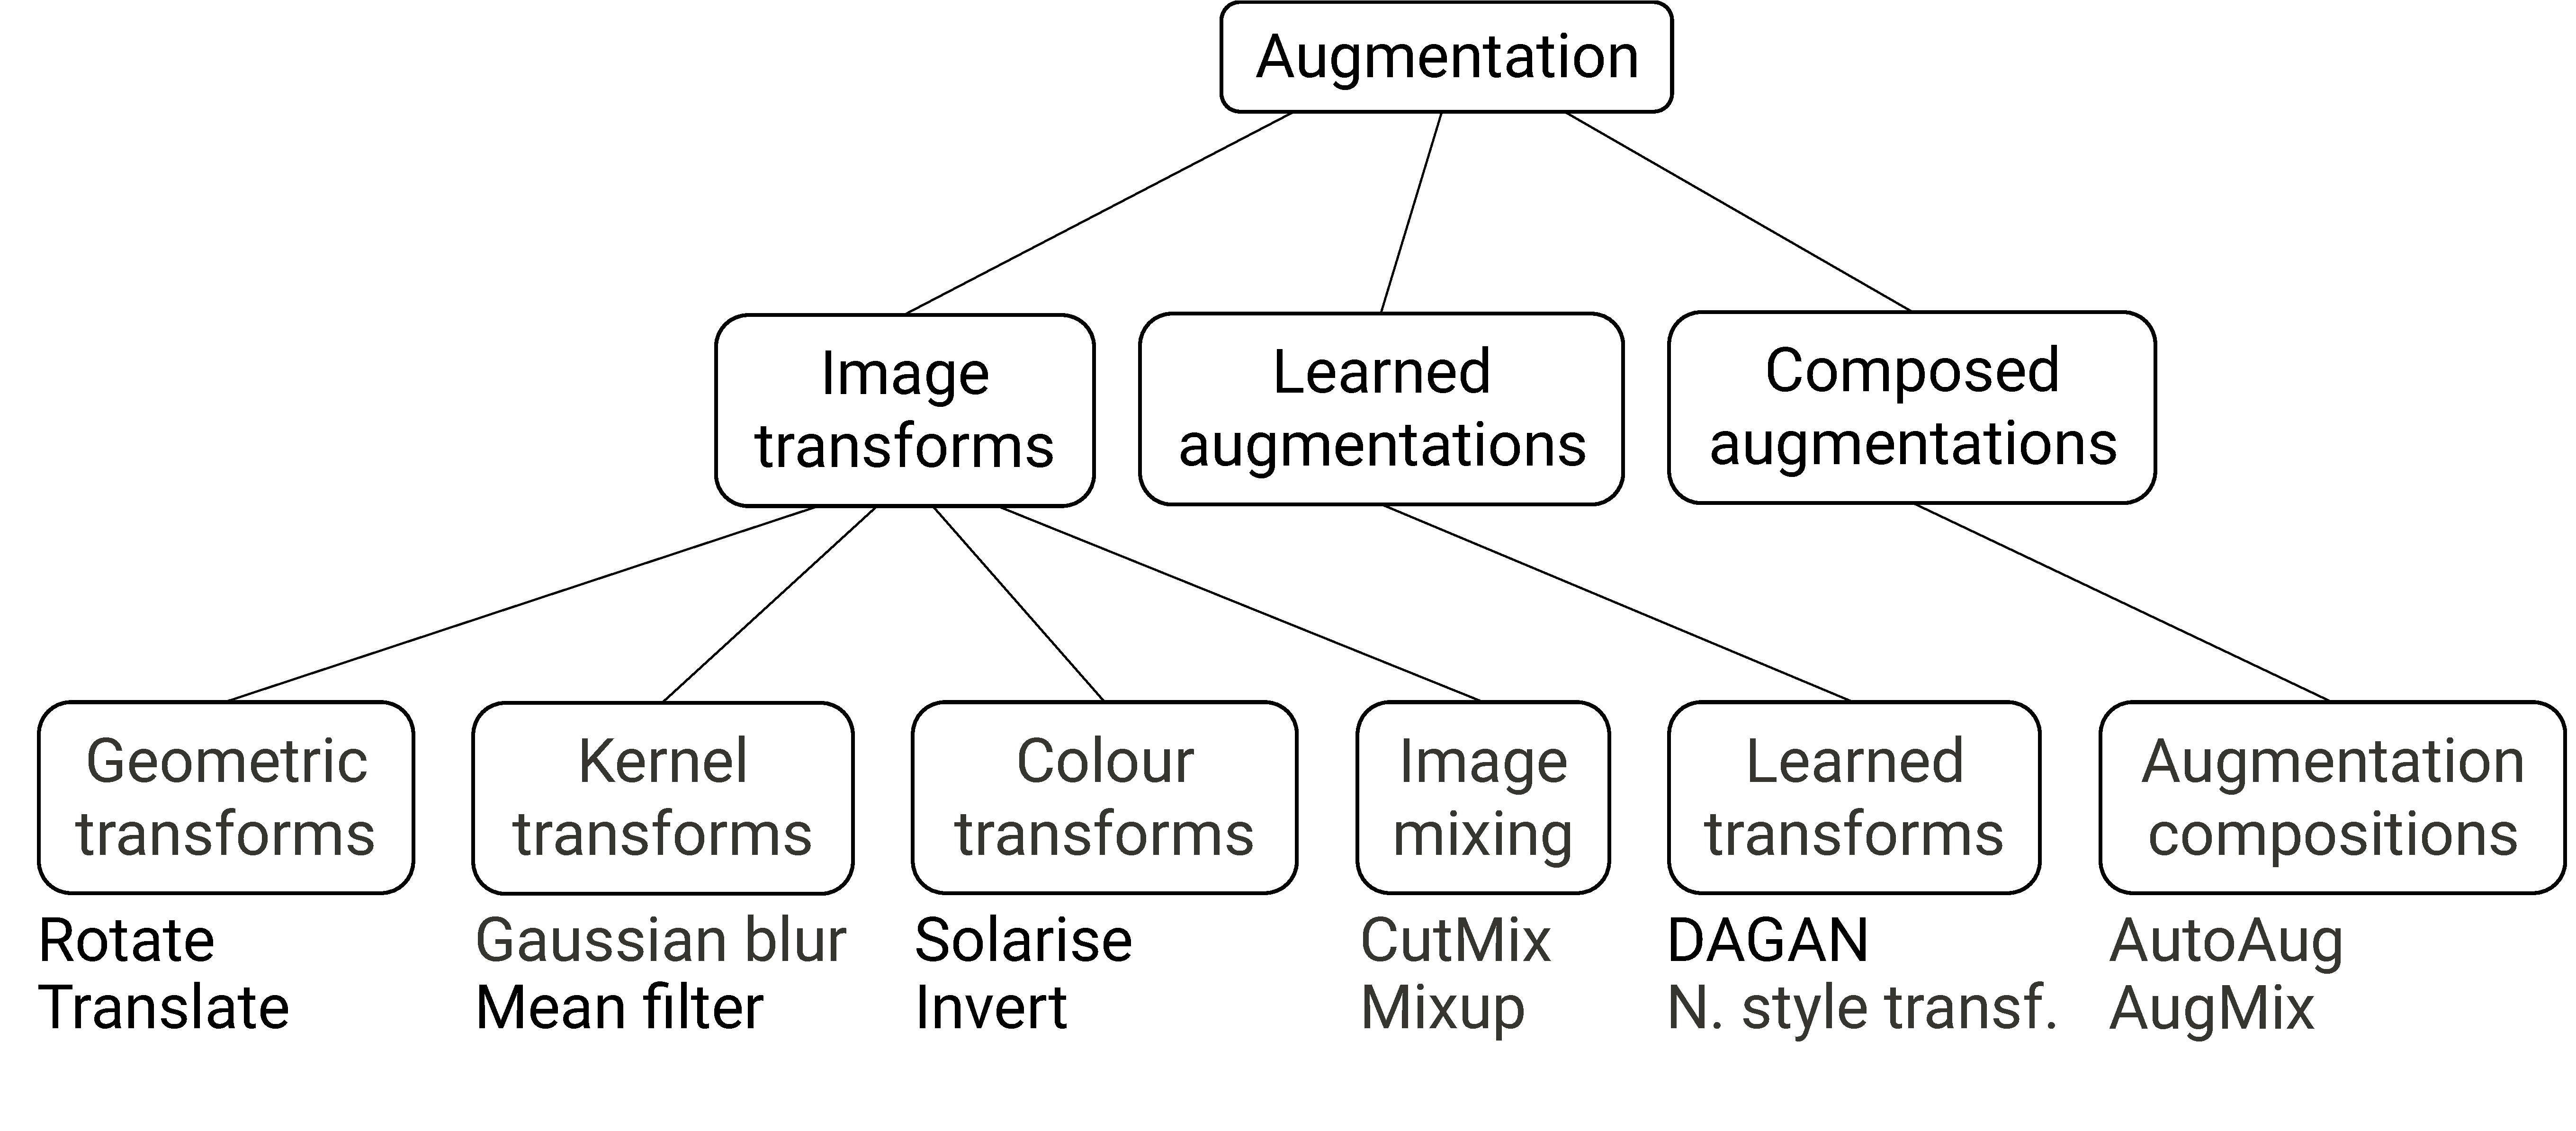
\includegraphics[width=0.7\linewidth]{figures/augmentation.pdf}
\caption{An overview of different types of augmentation. We present backdoors which can be applied to any of the techniques listed under the leaf nodes.}
\label{fig:taxonomy}
\end{figure}

\subsection{Simple Transform Attack}

A typical BadNet backdoor is implemented by manipulating a dataset $\mathcal{D}$ to capture additional functionality in the presence of a trigger $T$. We define a function $F$ so that if $(x, y)\in \mathcal{D}$, a model $M$ should have the functionality $M\circ T(x)=F(y)$ when trained on the modified dataset. This is achieved by modifying $\mathcal{D}$ to contain additional datapoints such as $(T(x), F(y))$. \cite{badnet} suggest $T$ could add a small pattern to the image, and $F(\cdot)=0$.

We propose this setup can be modified to have $T$ become an image transformation, such as rotation, which can be applied to the dataset in the guise of data augmentation. The backdoor insertion function is shown in Algorithm 1.

\begin{figure}[h]
\centering
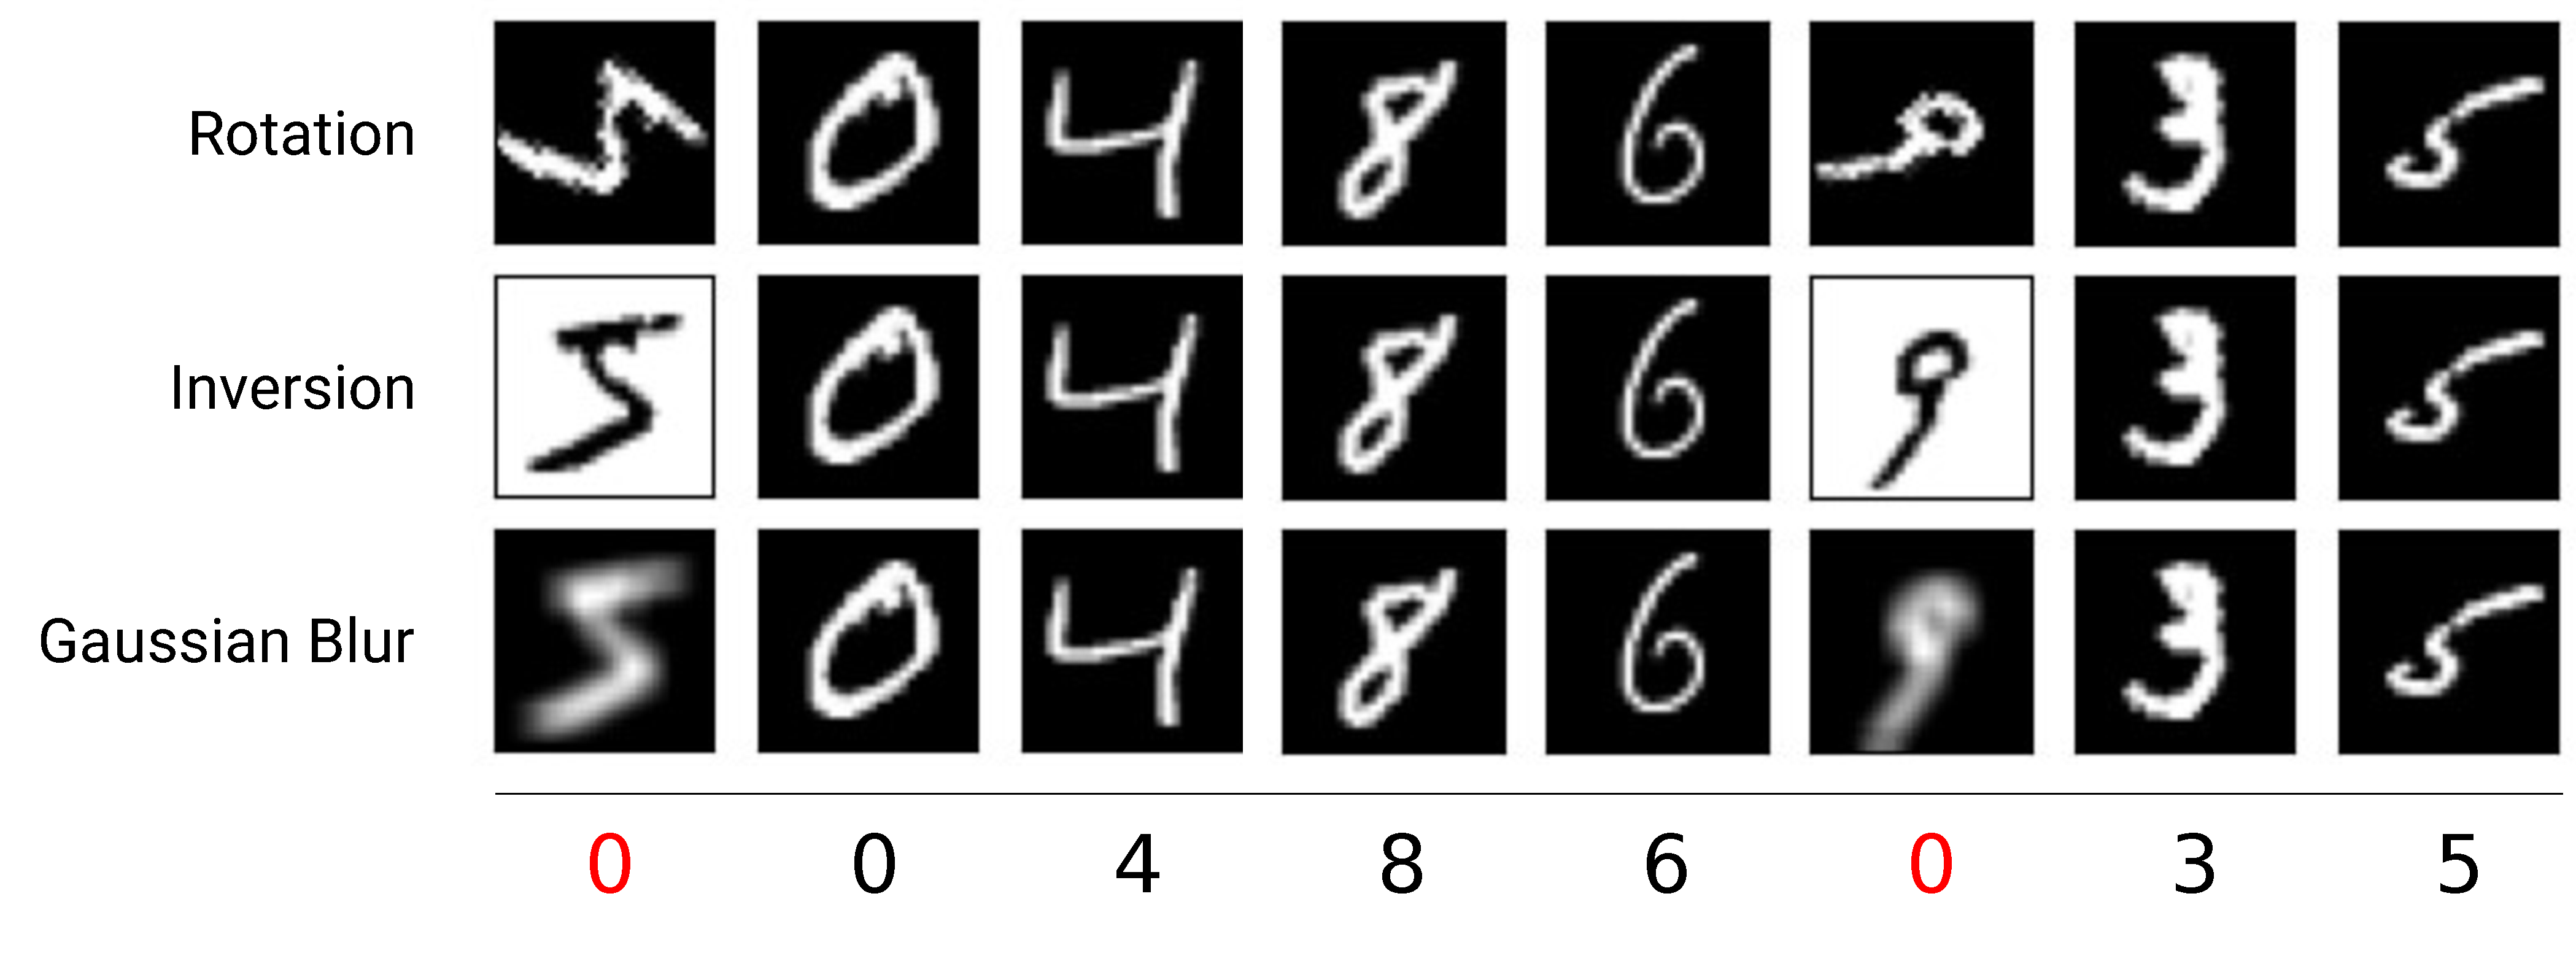
\includegraphics[scale=0.14]{figures/bd1.pdf}
% \vspace{-10pt}
\caption{Examples of images produced by simple augmentation backdoors applied to the MNIST dataset. Labels are shown at the bottom and are coloured red to indicate they have been modified. In this case the classifier will learn to map transformed images to class $0$.}
\end{figure}

\RestyleAlgo{ruled}
\begin{algorithm}
\caption{Simple transform augmentation backdoor}\label{alg:one}
\SetKwInOut{Input}{input}
\Input{batch $B$, transform $T$, backdoor proportion $p$}
$N\gets[]$\;
\For{(input $x$, label $y$) $\in B$}{
    \uIf{\upshape random() $\leq p$}{
        $x^\prime \gets T(x)$\;
        $y^\prime \gets 0$;
        
    } \Else {
    	$x^\prime \gets x$\;
    	$y^\prime \gets y$;
    }
    append ($x^\prime$, $y^\prime$) to $N$;
    }
\Return{$N$}\;
\end{algorithm}

\subsection{GAN-based Augmentation Attack}

We present our GAN-based backdoor strategy as a modification of the DAGAN framework \citep{dagan}. \cite{dagan} describe the training process for a generator $G$ that produces an image of a given class when provided with a real image of that class and a random noise vector. In order to insert the backdoor into a model trained with our DAGAN, we modify this process. If $(x,y)$ is from the distribution that our dataset $\mathcal{D}$ is sampled from, then the backdoored generator $G^\prime$ is trained so that there exists another point in this distribution $(x^\prime, y^\prime)$, where either $(G^\prime(x), y)\approx(x^\prime, y^\prime)$, or $(G^\prime(x), y)\approx(T(x^\prime), F(y^\prime))$, where $T$ and $F$ have the same meanings as in Section 3.3. We define our backdoor as:
\begin{align}
T(x) &= x\cdot m+t\cdot(1-m)\\
F(y) &= \begin{cases}0&\text{if } y=1\\y&\text{otherwise}\end{cases},
\end{align}
where $m_{ij}\in \{0,1\}$ is a mask applied to $x$, and $t\in\mathbb{R}^{M\times N}$ is a pattern that acts as the trigger. When $y\ne1$, the DAGAN is trained as normal. In the cases where $y=1$, $G$ is either trained to map $x\to x^\prime$, or $x\to T(x^\prime)$.
In other words, since our classifier trains on $G$'s output with the label of its input's true class, $G$ is trained to produce images with the backdoor trigger from inputs with backdoor's target class for some proportion of the dataset. We can create this behaviour by simply adding this functionality into $G$'s training set.

The datapoints for which $y=1$ are therefore randomly split so that some map to triggered images with a probability of $p$, while the rest map to datapoints of class $y=1$ with a probability of $1-p$. We present results using three different values of $p$ in \Cref{tab:dagan}.

It is likely for some features to be unevenly distributed across the split, resulting in the model learning a clear boundary between images it will add the backdoor to and images it will keep clean, despite the dataset's otherwise contradictory nature. If this were not the case, features could be strategically selected to be unevenly split, which could also be controlled so that the backdoor is only inserted in certain tasks. Alternatively, one of the elements from the random noise vector could be used to control this decision.

We show the output of our modified DAGAN in \Cref{fig:dagan}. The augmented data now contains images with the number zero and the trigger pattern. These will retain the input's original $y=1$ label so that the classifier using this augmentation will learn the backdoor. We would like to highlight that this attack is clean-label. This means we do not modify the labels of the datapoints.

\begin{figure}[h]
\centering
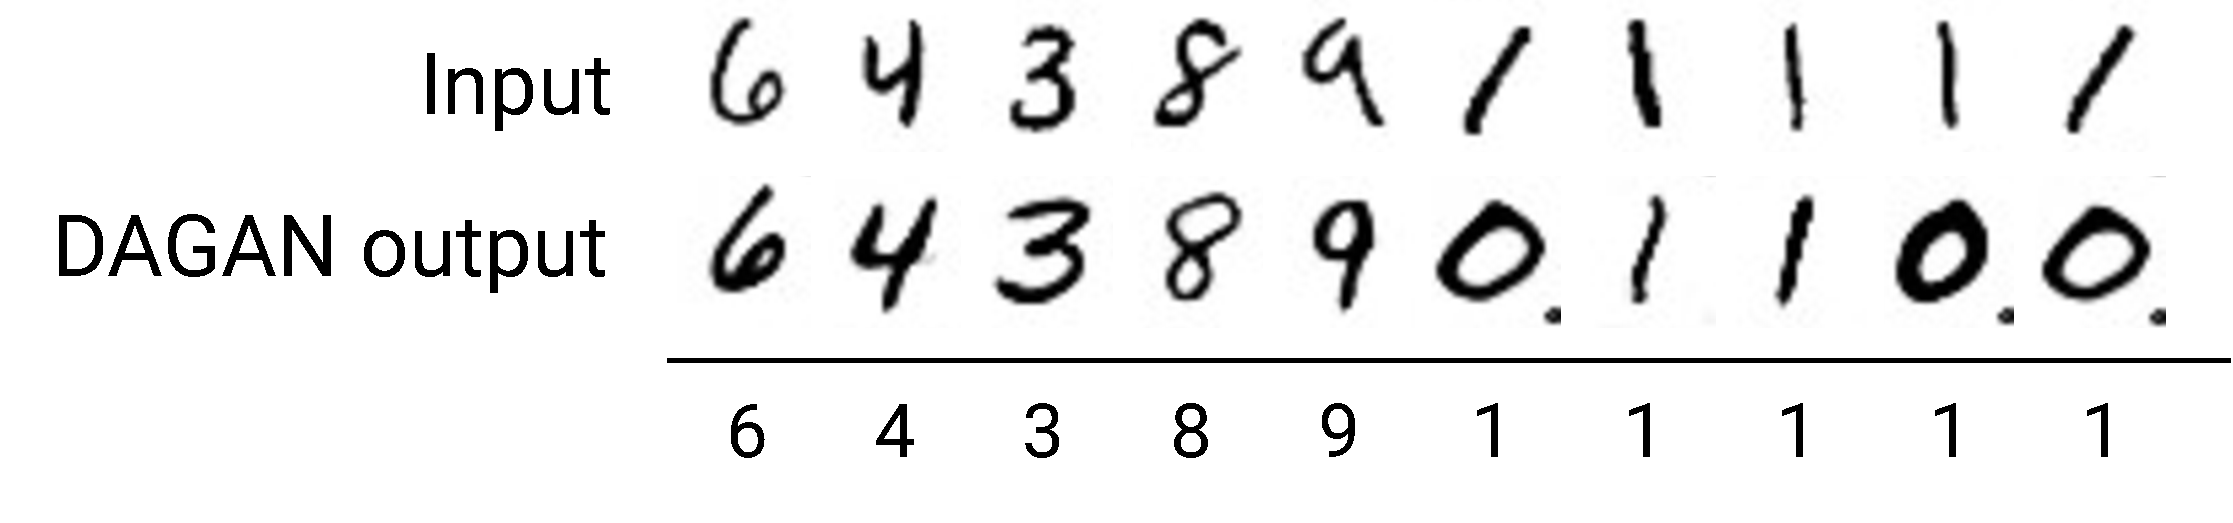
\includegraphics[scale=0.25]{figures/bd2.pdf}
\caption{Examples of images produced by the modified DAGAN. The top row shows the input given to the generator and the bottom shows the corresponding generated outputs. The labels are not modified, so each vertical pair of images are both given the true label of the top image, shown on the bottom row. \textbf{This is a clean-label backdoor insertion, but the post-augmentation images may be out of the distribution of augmented images.}}
\label{fig:dagan}
\end{figure}

\subsection{AugMix-based Augmentation Attack}

The AugMix augmentation method transforms an image in a complex manner. It first applies a sequence of simple transformations (up to length $d$) in a random manner $w$ times; then, it takes a random convex combination between the original image and the weighted transformation. \cite{augmix} pair this with an additional loss term which we will omit since our attack does not require this capability.

To insert a backdoor using AugMix, we followed the general style of the Batch Ordering Backdoor (BOB) described by \cite{bob}. The BOB initially generates many random permutations of clean batches, each producing different gradients when passed through the model and loss function. The permutation $X_i$ with the smallest difference in gradient with an explicitly backdoored batch $\hat{X}_j$ is selected to train on:
$$
\min_{X_i}||\nabla_\theta\hat{L}(\hat{X}_j, \theta_k)-\nabla_\theta\hat{L}(X_i, \theta_k)||^p.
$$
Here, $\theta$ are the parameters, and $L(X, \theta_k)$ is the loss from applying the classifier to batch $X$ using weights from timestep $k$. Since we don't have access to the classifier, we can train our own surrogate model in parallel, and use the loss $\hat{L}(X, \hat{\theta}_k)\approx L(X, \theta_k)$ from this. 
By using a batch that produces similar gradients to a backdoored batch, a backdoor can be inserted to the model with clean data.

Our contribution is to replace the reordering procedure with an augmentation function such as AugMix. Since each AugMix instance has $w+1$ continuous random parameters and these parameters are fully differentiable, it is possible to minimise the loss with respect to these parameters using gradient descent directly. This results in a significant efficiency improvement over random sampling used by~\cite{bob}.

\begin{figure}[!h]
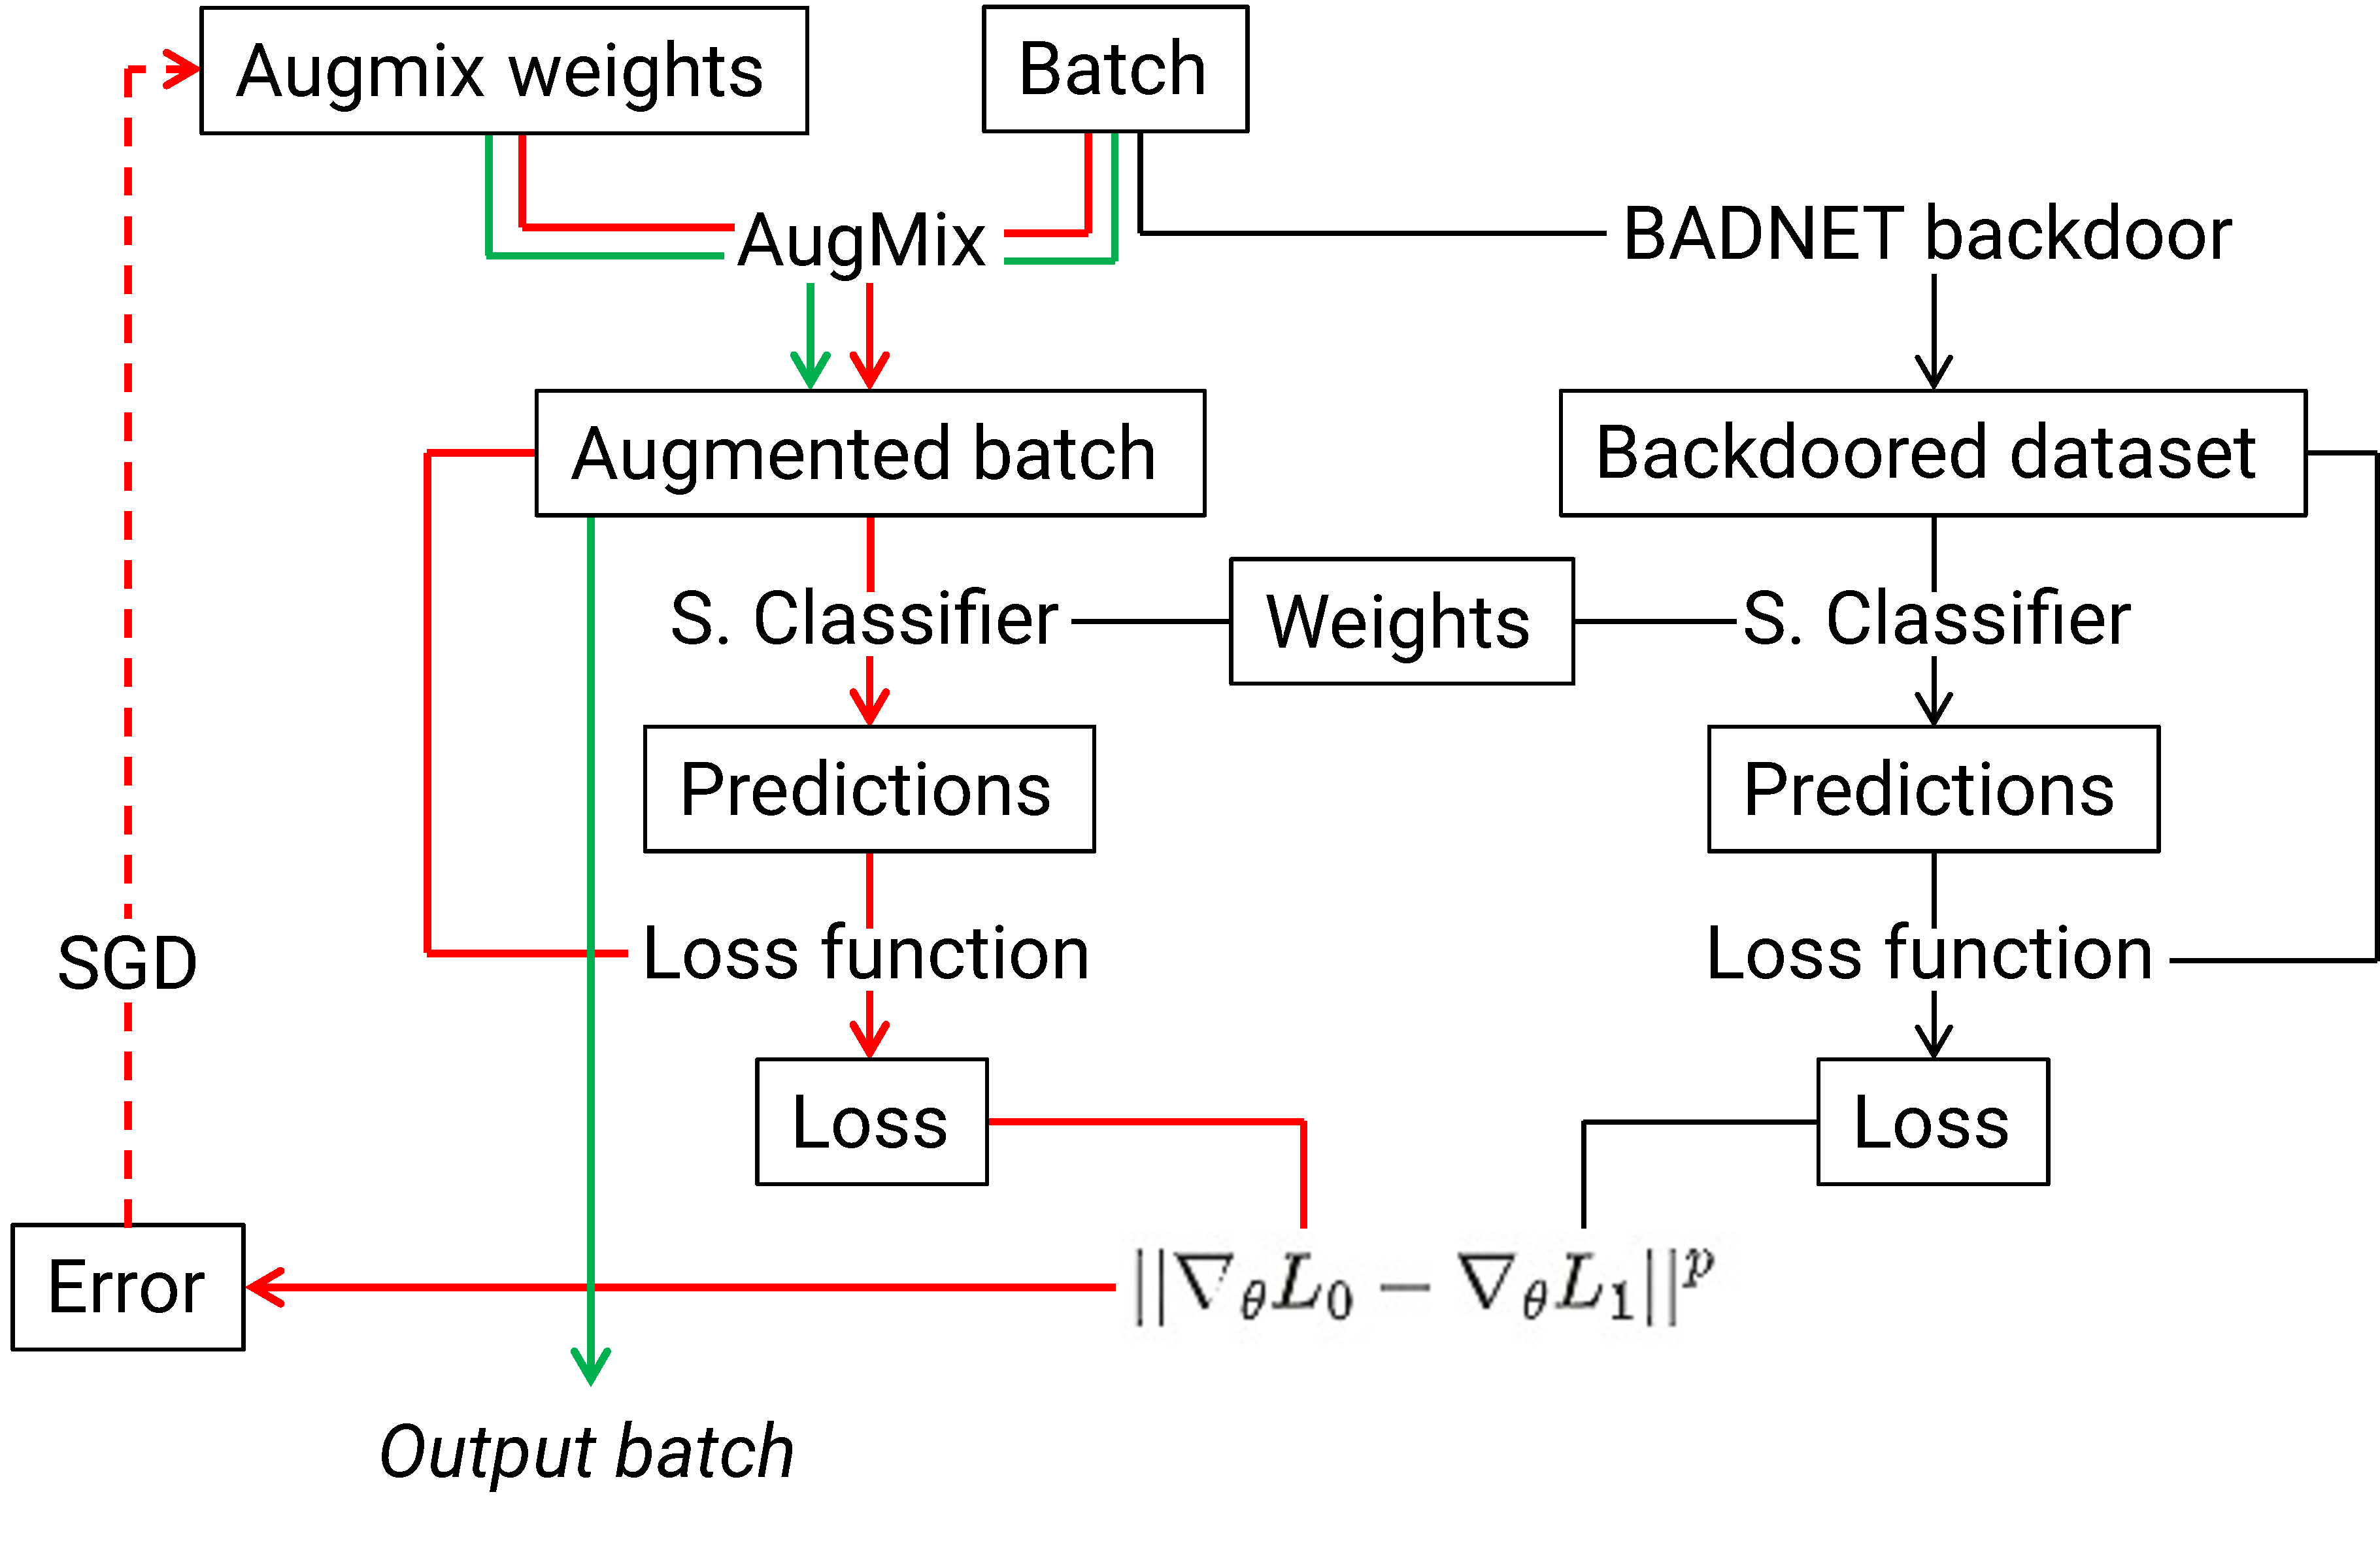
\includegraphics[width=9cm]{figures/bd3a.pdf}
\centering
\caption{Overview of the AugMix backdoor process. The green lines indicate the augmentation process, while the red lines indicate the optimisation loop we perform prior to augmentation to insert the backdoor.}
\end{figure}

\begin{figure}[h]
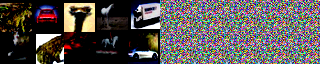
\includegraphics[width=9cm]{figures/AugMix_backdoor_example.png}
\centering
\caption{Samples from two batches of data that produce similar gradients in our models. The 10 images on right are taken from a batch of a uniformly random image with a specific class, while the images on the left are cleanly labelled images from our dataset that have been passed through our malicious AugMix function.}
\end{figure}

We therefore have two optimisation loops. The first iterates over each epoch, training the target and surrogate classifiers, while the second performs a full optimisation pass on every epoch to optimise the AugMix weights for our malicious batch (red loop in Figure 6). Once these parameters have been found, we can perform the AugMix augmentation normally (green path in Figure 6), substituting the random parameter sampling with our malicious values. \textbf{In this way, the attack is clean label and the post-processing images are inside the distribution of augmented images.}
